\section{Discussão}\label{sec:discussao}

Esta seção discute \textit{por que} o método é capaz de fazer o que os resultados mostram, e por que deixa de ser capaz em outros casos. As propriedades da construção são garantidas pela teoria, e o que se discute a seguir diz respeito, salvo menção contrária, à instanciação, isto é, a se uma escolha particular de fontes produz um espaço que reflete o modelo.

\subsection{A estrutura do espaço de representação, bloco a bloco}\label{subsec:disc_espaco}

Como a matriz de Gram é semidefinida positiva, cada objeto admite uma realização $\varphi_i$ com $G_{ij} = \langle \varphi_i, \varphi_j \rangle$ (Equação \eqref{eq:empirical_feature_realization}), e as coordenadas associadas aos dois maiores autovalores, $\bigl(\sqrt{\hat\lambda_1}\,V_{i1}, \sqrt{\hat\lambda_2}\,V_{i2}\bigr)$, formam a projeção plana que preserva a maior parte da energia do espaço, sem nenhum parâmetro adicional. A Figura \ref{fig:disc_espaco} mostra essa projeção em todos os blocos do perceptron multicamadas treinado sobre a base \texttt{segment}, que tem sete classes, poucas o bastante para serem distinguidas por cor.

\begin{figure}[htbp]
  \centering
  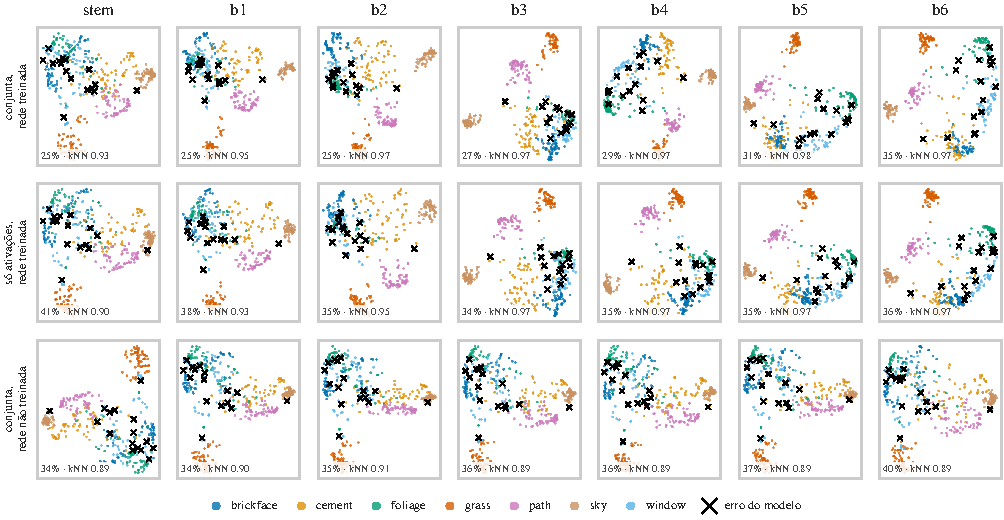
\includegraphics[width=\textwidth]{figuras/disc_espaco.pdf}
  \caption{O espaço de representação bloco a bloco, projetado nos seus dois modos dominantes, sobre as 462 amostras de teste da \texttt{segment} (perceptron multicamadas, semente 0, alvo fixo). A primeira linha mostra a Gram conjunta da rede treinada, a segunda apenas a fonte de ativações, com a mesma transformação das componentes, e a terceira a Gram conjunta da rede não treinada, com os mesmos pesos iniciais. A cor é a classe predita pela rede treinada, e os $\times$ marcam as amostras que ela erra. No canto de cada painel estão a fração da energia retida pelos dois eixos e o acerto do $k$-vizinhos contra a predição, calculado sobre a matriz de Gram inteira, e não sobre o plano.}
  \label{fig:disc_espaco}
\end{figure}

Três aspectos da figura ajudam a entender os resultados. O primeiro é o contraste entre a rede treinada e a não treinada. Na rede não treinada (terceira linha), a geometria é praticamente a mesma em todos os blocos: a rede aleatória apenas propaga a estrutura da entrada, e as classes que já são separáveis nos atributos brutos, como \texttt{grass} e \texttt{sky}, aparecem isoladas desde o \texttt{stem}. É exatamente essa separabilidade herdada da entrada que torna o piso cruzado alto nas bases tabulares, com $k$-vizinhos em torno de $0{,}89$ nesta base. Na rede treinada (primeira linha), ao contrário, a geometria muda a cada bloco: \texttt{path}, \texttt{grass} e \texttt{sky} se destacam em grupos compactos a partir de \texttt{b3}, e as classes que a rede tem mais dificuldade de separar, \texttt{brickface}, \texttt{foliage}, \texttt{window} e \texttt{cement}, passam a ocupar uma região comum. O que distingue a medida do seu piso é, portanto, a reorganização produzida pelo treinamento, e não a separabilidade dos dados.

O segundo aspecto é a posição dos erros. Os objetos que o modelo erra não estão espalhados pelo espaço: eles se concentram na região em que as classes confundíveis se encontram, e isso ocorre em todos os blocos da rede treinada. Essa é a razão pela qual a margem geométrica prevê o acerto (P1). Um objeto cuja vizinhança mistura predições diferentes está, geometricamente, em uma fronteira, e é nas fronteiras que o modelo erra. Veja que o método não recebe o rótulo verdadeiro em nenhum momento, de modo que essa concentração é uma propriedade do espaço construído, e não da forma como ele foi desenhado.

O terceiro aspecto é a comparação entre a composição e a fonte de ativações isolada (segunda linha). Nesta base tabular, as duas geometrias são parecidas, e a composição só se distingue nos blocos rasos, o padrão que P2 encontrou nas bases tabulares. Por fim, é preciso ler a figura com uma cautela: os dois eixos retêm apenas de 25\% a 40\% da energia, de modo que objetos sobrepostos no plano podem estar separados nas demais dimensões, e é por esse motivo que o acerto do $k$-vizinhos é calculado sobre a matriz inteira.

\subsection{O que o método é capaz de fazer, e por quê}\label{subsec:res_instanciacao}

\textbf{Refletir a decisão e o erro.} A primeira capacidade demonstrada é a de construir um espaço em que a vizinhança de um objeto antecipa como o modelo o trata. A razão está na forma multiplicativa da composição. Como discutido no Comentário \ref{rem:joint_similarity}, o produto de Hadamard impõe um critério de similaridade conjunta: dois objetos só são próximos se forem próximos em todas as fontes simultaneamente. Na instanciação utilizada, isso significa que dois objetos vizinhos têm estados parecidos, ativam filtros parecidos \textit{e} têm a decisão sensível às mesmas direções. Vizinhos nesse espaço compartilham, portanto, não apenas o conteúdo, mas a razão pela qual o modelo os trataria da mesma forma, e é essa propriedade que permite usar a vizinhança como indício de confiança, como fazem o \textit{trust score} e os $k$-vizinhos profundos \citep{Jiang2018, Papernot2018}.

\textbf{Acrescentar algo às ativações onde elas ainda não decidem.} A composição supera a fonte de ativações nos blocos rasos e intermediários e se iguala a ela na saída da rede, e a diferença é muito maior na ResNet do que no perceptron multicamadas. A explicação é que as ativações descrevem o que a rede \textit{vê}, enquanto o gradiente contrastivo descreve o que \textit{importaria} para a decisão. Nos blocos profundos, as ativações das amostras de uma mesma classe tendem a colapsar em torno de uma média de classe \citep{Papyan2020} e passam a carregar a decisão por si mesmas, de modo que a composição deixa de ter o que acrescentar. No perceptron multicamadas, cuja entrada já é quase separável, e no transformador, cujo gradiente quase não carrega informação sobre a decisão, a vantagem é pequena ou inexistente. Veja que isso delimita a instanciação, e não o método: a contribuição de cada fonte é uma propriedade do modelo analisado, e outra escolha de fontes pode ser mais informativa em outra arquitetura.

\textbf{Ver o que a CKA não vê.} A decomposição contra a CKA mostrou que a parte da Gram vista pela CKA coincide com a geometria euclidiana das ativações, de modo que a parte residual é exatamente o que uma análise das ativações não enxerga. Essa parte residual prevê o acerto melhor do que a vista nos blocos rasos e intermediários da ResNet e pior nas bases tabulares e no transformador. Veja que esse é o mesmo padrão da capacidade anterior, e pela mesma razão: o que o método vê além da CKA é, essencialmente, a contribuição do gradiente. Sendo assim, o método se distingue da CKA exatamente onde a sensibilidade da decisão diverge do conteúdo das ativações.

\textbf{Concentrar a decisão em poucas direções.} A leitura espectral mais robusta é a contenção das direções de classe no subespaço retido, em que a composição supera as ativações em toda a profundidade, nas bases tabulares e nas duas arquiteturas. Isso significa que as poucas direções dominantes do espaço construído são as direções em que o modelo separa as suas decisões. A razão de energia ortogonal, que mede quanto de cada objeto vive fora dessas direções, só é confiável quando o subespaço retido já é o subespaço da decisão, isto é, nos blocos profundos da ResNet e em quase todos os blocos do transformador. Em outras palavras, a energia que escapa de $V_r$ sinaliza uma amostra que o modelo não sabe representar apenas quando $V_r$ é o espaço em que o modelo decide, a mesma condição que torna útil o resíduo do subespaço principal na detecção de amostras fora da distribuição \citep{Wang2022ViM}.

\textbf{Localizar sem necessariamente explicar.} Sobre a entrada, o campo de energia da ResNet localiza o animal muito melhor do que um mapa centrado e do que o Grad-CAM, mas ordena a evidência da decisão pior do que o Grad-CAM nos blocos profundos. A diferença entre as duas tarefas explica o resultado. A energia de uma posição mede o quanto ela participa dos modos dominantes da geometria da imagem, isto é, da estrutura que o modelo representa, enquanto o Grad-CAM pondera cada posição diretamente pela sensibilidade da decisão. Um mapa de estrutura cobre o objeto inteiro, enquanto um mapa de sensibilidade ordena as suas partes pela importância. No transformador, nem a localização se sustenta, porque a atenção mistura informação de toda a imagem desde as primeiras camadas \citep{Raghu2021}, e a posição deixa de ser uma unidade natural de objeto. Na prática, o campo de energia é útil para auditar \textit{onde} uma rede convolucional representa o objeto, por exemplo para detectar um modelo que se apoia no fundo \citep{Geirhos2020}, mas não substitui um mapa de relevância quando a pergunta é quais partes sustentam a decisão.

\textbf{Explicar por contrafactuais, inclusive fora das redes neurais.} A leitura de pares responde à pergunta contrastiva, ``por que esta amostra e não aquela?'', que é a forma natural das explicações humanas \citep{Miller2019}, e o faz tomando como referência um contrafactual no sentido de \cite{Guidotti2022}: a amostra observada mais próxima que o modelo decide de outra forma. A distância do método entra em dois pontos. Ela ordena as diferenças entre a amostra e o seu contrafactual pelo quanto cada uma aproxima as duas no espaço do modelo, e cada pontuação $\Delta d_f$ é o efeito de uma intervenção $do(x_f := x_{j,f})$ sobre essa distância. É por isso que o método supera o SHAP e o LIME nas formas em que eles são usualmente aplicados, que explicam uma amostra em relação a uma referência genérica, e não em relação ao contrafactual. O resultado mais forte, entretanto, vem da árvore de decisão, em que a resposta certa é conhecida e o método a recupera sem receber a regra de decisão, apenas trocando as fontes. Esse é o argumento mais direto de que o método é modelo-agnóstico: a construção exige somente que cada amostra possa ser descrita por fontes sobre as quais se define um \textit{kernel}, e o que depende do modelo é apenas a instanciação.

\textbf{Datar a decisão.} As leituras por bloco produzem uma datação da decisão, e nas redes essa datação concorda com a obtida por intervenção sobre os estados internos. Essa concordância, contudo, decorre em boa parte de as duas séries crescerem com a profundidade, e por isso ela não é, sozinha, uma validação. A validação veio da árvore, em que a profundidade da decisão é conhecida para cada par. Uma consequência prática é que a leitura por bloco permite localizar em que ponto da rede uma distinção passa a ser usada, como no par da \texttt{letter} em que a dispersão horizontal da letra só pesa no meio da rede, uma informação que atribuições sobre a saída do modelo não oferecem.

\subsection{Quando o método não é capaz, e por quê}\label{subsec:disc_limites}

Três limites decorrem da própria construção das leituras, e não de detalhes de implementação.

O primeiro é que a leitura de pares é de primeira ordem. A pontuação $\Delta d_f$ intervém em um atributo de cada vez, e os atributos que só importam em conjunto não mudam nada quando trocados sozinhos. Por isso o método recupera o atributo que separa a amostra do seu contrafactual, mas não o contrafactual mínimo, isto é, o menor conjunto de mudanças que altera a decisão, e o valor de Shapley com $j$ de referência, que considera todas as combinações de trocas, o supera no teste de trocas. Em outras palavras, o método explica o que distingue duas instâncias, e não como transformar uma na outra com o menor custo, que é o objetivo dos geradores de contrafactuais \citep{Wachter2018, Guidotti2022}. Uma extensão natural do método é substituir a troca isolada por trocas sequenciais, recalculando a distância depois de cada uma, o que capturaria interações e manteria o custo linear no número de atributos.

O segundo é que o método depende de o treinamento reorganizar a geometria. Se a tarefa é resolvida quase na entrada, a rede treinada e a não treinada produzem espaços parecidos, e as leituras se aproximam do que a diferença bruta entre as amostras já dizia. É o que se observa nas bases tabulares, em que o piso cruzado é alto e a leitura de pares empata com a diferença bruta $|\Delta x|$, e é coerente com a Figura \ref{fig:disc_espaco}, em que a vantagem sobre o piso é justamente a reorganização entre os blocos. A similaridade entre a Gram da rede treinada e a da rede na inicialização é barata e poderia ser reportada antes de qualquer leitura, como um diagnóstico de aplicabilidade, mas esse critério ainda precisa ser validado sobre um número maior de bases.

O terceiro é que a validade das leituras referidas à decisão depende da escolha do alvo do gradiente. Com a classe predita como alvo, o gradiente carrega a própria predição, e as leituras de decisão se tornam circulares, chegando a recuperar a predição em mais de 95\% dos casos já em \texttt{b3} da ResNet. O alvo fixo remove essa circularidade ao custo de tornar o gradiente degenerado no último bloco. Essa é uma restrição da fonte de gradiente, e não do método, mas qualquer instanciação que utilize a decisão como fonte precisa de um controle equivalente.

\subsection{Limitações e trabalhos futuros}\label{subsec:res_limitacoes}

A proposição de que as distâncias do espaço de representação refletem o entendimento que o modelo tem dos dados foi avaliada apenas em sua dimensão comportamental. Nenhuma referência semântica externa ao modelo, como uma hierarquia de superclasses ou julgamentos humanos de similaridade, foi utilizada, de modo que a afirmação de que as distâncias representam diferenças semânticas permanece sem teste.

Do ponto de vista experimental, quatro limitações devem ser registradas. A base de imagens impõe um regime de dados escassos, com cerca de noventa imagens por raça, o que limita a acurácia dos modelos treinados do zero, sobretudo a do transformador. Treinar a partir de pesos pré-treinados elevaria essa acurácia, mas descaracterizaria o piso, que é a mesma rede na inicialização. As comparações são reportadas pela média, pelo desvio e pela fração das execuções em que se sustentam, sem testes de hipótese. Testes pareados ao nível dos pares, como o de postos sinalizados de Wilcoxon com correção para comparações múltiplas, e o teste de Friedman entre bases seriam os adequados a este desenho. A leitura de previsão do acerto não foi comparada à confiança do próprio \textit{softmax}, e os estudos de caso utilizam uma única base. Por fim, os conjuntos de nível foram validados apenas na ResNet, o piso adotado na diagonal da transformação angular não foi variado e a seleção da posição de referência ainda não exclui a borda da imagem.

Além das extensões já mencionadas, a leitura de pares por trocas sequenciais e a decomposição espectral truncada para amostras maiores, duas direções decorrem diretamente da separação entre método e instanciação. A primeira é explorar outras fontes para as arquiteturas em que o gradiente pouco contribui, como o transformador, em que a atenção é uma candidata natural a fonte. A segunda é utilizar o método para comparar modelos diferentes sobre as mesmas amostras, como a árvore de decisão e o perceptron multicamadas da \texttt{letter}, colocando os dois na mesma geometria e perguntando não apenas se eles usam os mesmos atributos, mas se organizam os dados da mesma forma.
